\chapter{KIẾN THỨC HỆ THỐNG}

\section{Cơ sở lý thuyết của kiến trúc}

\subsection{Kiến trúc Modular}

Kiến trúc Modular là kiểu kiến trúc phần mềm cho phép quản lý sự phức tạp của một vấn đề bằng cách chia nhỏ chúng thành các Modular để dễ quản lý hơn với các nguyên tắc và mô hình. Modular là một đơn vị phần mềm không trạng thái có thể triển khai, quản lý, tái sử dụng, kết hợp lại và cung cấp giao diện ngắn gọn cho người dùng.

Khi phát triển phần mềm, khi hệ thống càng lớn thì càng cần thêm nhiều component, dẫn tới sự thay đổi nhỏ trong một component có thể ảnh hưởng tới nhiều component khác. Trong hệ thống, module là những component được phát triển bên ngoài ứng dụng. Module giao tiếp với ứng dụng thông qua entry-point.

\begin{figure}[H]
	\centering
	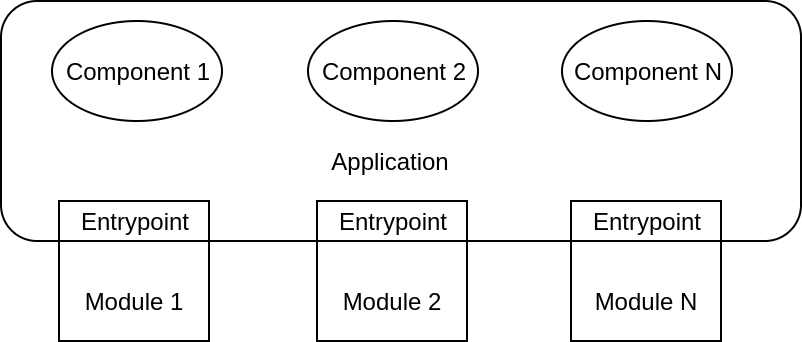
\includegraphics[width = 1\textwidth]{modules}
	\caption{Kiến trúc Modular}
\end{figure}

Sử dụng kiến trúc Modular đem lại một số lợi ích:

\begin{itemize}
	\bfitem{Tùy chỉnh}{ứng dụng có thể hoạt động thực sự khác biệt bằng cách chỉ bật / tắt một số Modular.}
	\bfitem{Ít phụ thuộc hơn}{các Modular độc lập hơn với chính ứng dụng, cho đến khi các "điểm vào" tương thích, cả Modular và ứng dụng có thể phát triển độc lập.}
	\bfitem{Các phần mở rộng của bên thứ ba}{vì các Modular không phải là một phần của ứng dụng và các "điểm vào" được xác định rõ, việc phát triển các Modular có thể được thực hiện bởi các bên thứ ba.}
	\bfitem{Phát triển độc lập}{Vì ứng dụng và các Modular là độc lập, chúng có thể là:}
	\begin{itemize}
		\item được phát triển bởi các nhà phát triển bên ngoài
		\item phát hành với các chu kỳ phát hành độc lập
		\item được phát triển tiềm năng với các công nghệ khác nhau
	\end{itemize}
	\bfitem{Ứng dụng nhỏ hơn}{Các ứng dụng nhỏ hơn (nhiều chức năng có thể được thực hiện thông qua các Modular) và ứng dụng nhỏ hơn được dịch để có khả năng bảo trì tốt hơn.}
\end{itemize}

Modular được hình thành dựa trên việc nhóm những lớp có mức độ liên quan cao thành một Modular để có tính tương liên cao nhất. Có 2 loại tương liên:

\begin{itemize}
	\item Tương liên giao tiếp: có được khi 2 phần của Modular thao tác trên cùng dữ liệu.
	\item Tương liên chức năng: có được khi mọi phần của Modular làm việc cùng nhau để thực hiện tác vụ định rõ.
\end{itemize}

\subsection{Domain Driven Design}

Domain-Driven Design là một phương pháp hay cách thức tiếp cận trong việc phân tích và phát triển phần mềm trong khi giải quyết những vấn đề nghiệp vụ phức tạp. Ý tưởng cơ bản của cách thức này là việc xây dựng sự kết nối chặt chẽ giữa thiết kế phần mềm và mô hình nghiệp vụ trong suốt vòng đời phát triển sản phẩm. 

Để tạo nên sự kết nối này, Eric Evans đã đưa ra khái niệm này vào năm 2004, trong cuốn sách Domain-Driven Design: Tackling Complexity in the Heart of Software. Theo cuốn sách, nó tập trung vào ba nguyên tắc:

\begin{itemize}
	\item Trọng tâm của dự án là những nguyên tắc và logic nghiệp vụ
	\item Các thiết kế phức tạp dựa trên các mô hình nghiệp vụ.
	\item Sự hợp tác giữa các chuyên gia kỹ thuật và miền là rất quan trọng để tạo ra một mô hình ứng dụng giải quyết các vấn đề cụ thể trong mô hình nghiệp vụ.
\end{itemize}

Khi các đoạn code liên quan đến nghiệp vụ được trộn lẫn giữa các tầng lại với nhau, nó trở nên vô cùng khó khăn cho việc đọc cũng như suy nghĩ về chúng. Các thay đổi ở giao diện người dùng cũng có thể thực sự thay đổi cả logic nghiệp vụ. Để thay đổi logic nghiệp vụ có thể yêu cầu tới truy vết tỉ mỉ các đoạn mã của giao diện người dùng, CSDL, hoặc các thành phần khác của chương trình. Mô hình phát triển hướng đối tượng trở nên phi thực tế. Do đó, hãy phân chia một chương trình phức tạp thành các tầng. Phát triển một thiết kế cho mỗi tầng để chúng trở nên gắn kết và chỉ phụ thuộc vào các tầng bên dưới. Dưới đây là giải pháp kiến trúc chung cho DDD.

Ở đây mô hình DDD vẫn giữ lại những ưu điểm của mô hình kiến trúc phân lớp (Layered Archiecture) để đảm bảo nguyên lý Seperation of Concerns. Các phần logic xử lý khác nhau sẽ được cô lập ra khỏi các phần khác làm tăng tính Lose Coupling của ứng dụng và tính dễ đọc và dễ bảo trì cũng như ứng dụng khi có thay đổi logic của từng tầng thì không ảnh hướng đến các tầng khác.

Tác giả Eric Evan đề xuất kiến trúc đa tầng bao gồm:

\subsubsection{Tầng Application}

Tầng này không chứa logic nghiệp vụ. Đó là phần dẫn người dùng từ giao diện này đến giao diện khác. Nó cũng tương tác với các tầng Application của các hệ thống khác. Nó có thể thực hiện xác nhận đơn giản nhưng nó không chứa logic liên quan đến nghiệp vụ hoặc quyền truy cập dữ liệu. Mục đích của nó là tổ chức và ủy quyền các đối tượng nghiệp vụ thực hiện công việc của chúng.

\subsubsection{Tầng Domain}

Đây là nơi chứa các khái niệm về lĩnh vực nghiệp vụ. Tầng này có tất cả thông tin về trường hợp nghiệp vụ và các quy tắc nghiệp vụ. Đây là vị trí của các thực thể, ví dụ như người dùng hoặc sản phẩm.

Quan trọng nhất, tầng này phải nằm ở trung tâm, điều này có nghĩa là nó nên được tách biệt với phần còn lại của các tầng. Nó không nên phụ thuộc vào các tầng khác hoặc khuôn khổ của chúng.

\subsubsection{Tầng Infrastructure}

Tầng Infrastructure làm việc trực tiếp với hạ tầng công nghệ của hệ thống phần mềm. Các chức năng chính của tầng này bao gồm:

\begin{itemize}
	\item Truy vấn, thay đổi thông tin trong cơ sở dữ liệu
	\item Quản lý dữ liệu trên vùng nhớ tạm thời (cache data)
	\item Bảo mật, giám sát, lưu trữ thông tin hoạt động (log, monitor)
\end{itemize}

Tầng này đóng vai trò như một thư viện hỗ trợ cho tất cả các tầng còn lại. Nó cung cấp thông tin liên lạc giữa các lớp, cung cấp chức năng lưu trữ các đối tượng nghiệp vụ, chứa các thư viện hỗ trợ cho tầng giao diện người dùng...

\begin{figure}[H]
	\centering
	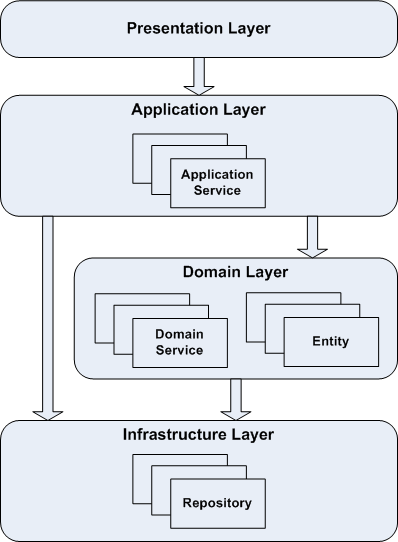
\includegraphics[height = 0.5\textwidth]{ddd-layer}
	\caption{Các tầng trong DDD}
\end{figure}

Domain-Driven Design chứa các khuôn mẫu (building blocks) có mục đích là để trình bày một số yếu tố chính của mô hình hóa hướng đối tượng và thiết kế phần mềm từ quan điểm của DDD.

Các khuôn mẫu cơ bản được sử dụng trong DDD gồm: Entities, Service, Value Object, Repository và Aggregate.

\subsubsection{Entities}

Trong các đối tượng của một phần mềm, có một nhóm các đối tượng có định danh riêng. Đối với những đối tượng này thì các thuộc tính của chúng có giá trị như thế nào không quan trọng bằng việc chúng tồn tại liên tục và xuyên suốt quá trình của hệ thống, thậm chí là sau cả khi đó. Chúng được gọi tên là thực thể - Entity.

Các Entities là sự kết hợp của dữ liệu và hành vi, như người dùng hoặc sản phẩm. Chúng có danh tính, nhưng đại diện cho các điểm dữ liệu với hành vi.

Lấy ví dụ, để tạo một lớp Person chứa thông tin về một người chúng ta có thể tạo Person với các trường như: tên, ngày sinh, nơi sinh v.v... Những thuộc tính này có thể coi là định danh của một người không? Tên thì không phải vì có thể có trường hợp trùng tên nhau, ngày sinh cũng không phải là định danh vì trong một ngày có rất nhiều người sinh ra, và nơi sinh cũng vậy. Một đối tượng cần phải được phân biệt với những đối tượng khác cho dù chúng có chung thuộc tính đi chăng nữa. Việc nhầm lẫn về định danh giữa các đối tượng có thể gây lỗi dữ liệu nghiêm trọng.

Đối với một người đó có thể là một tổ hợp của các thông tin như: tên, ngày sinh, nơi sinh, tên bố mẹ, địa chỉ hiện tại... Đối với một tài khoản ngân hàng thì số tài khoản là đủ để tạo định danh. Điểm mấu chốt ở đây là hệ thống có thể phân biệt hai đối tượng với hai định danh khác nhau một cách dễ dàng, hay hai đối tượng chung định danh có thể coi là một.

\begin{figure}[H]
	\centering
	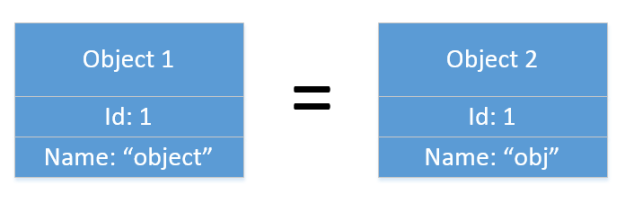
\includegraphics[width = 1\textwidth]{entity}
	\caption{Khuôn mẫu Entity}
\end{figure}

\subsubsection{Value objects}

Một đối tượng mà được dùng để mô tả các khía cạnh cố định của một domain, và không có định danh, được gọi tên là Value Object.

Value Object thể hiện những thành phần hoặc khái niệm của domain mà chỉ được biết bằng đặc điểm của nó. Chúng được dùng như mô tả của thành phần trong model, và không yêu cầu định danh. Value Object không cần định danh bởi vì chúng luôn kết hợp với một đối tượng khác và do đó luôn có thể hiểu được trong ngữ cảnh cụ thể.

Một điểm quan trọng là Value Object được xem như là bất biến, và không bao giờ được thay đổi trong vòng đời của mình. Ưu điểm của nó là nhờ không có định danh nên có thể tạo và xóa dễ dàng.

Value object có các thuộc tính, nhưng không thể tự tồn tại. Ví dụ: địa chỉ giao hàng có thể là một value object. Các hệ thống lớn và phức tạp có vô số entitiy và value object. Đó là lý do tại sao mô hình miền cần một số loại khuôn mẫu tiếp theo. Điều này sẽ đưa chúng vào các Aggregates hợp lý sẽ dễ quản lý hơn.

\subsubsection{Aggregates}

Những nhóm này được gọi là Aggregates. Chúng đại diện cho một tập hợp các đối tượng được kết nối với nhau, với mục tiêu coi chúng như các đơn vị. Hơn nữa, chúng cũng có một aggregate root. Đây là thực thể duy nhất mà bất kỳ đối tượng nào bên ngoài tổng thể đều có thể tham chiếu đến.

Entity và Value Object hình thành nên những mối quan hệ phức tạp trong domain model. Khi hệ thống lớn và có sự kết nối, tương tác giữa nhiều đối tượng, việc đảm bảo tính tương tranh và nhất quán trở nên khó khăn.

Do vậy, chúng ta cần sử dụng Aggregate. Một Aggregate là một nhóm các đối tượng, nhóm này có thể được xem như là một đơn vị thống nhất đối với các thay đổi dữ liệu. Một Aggregate được phân tách với phần còn lại của hệ thống, ngăn cách giữa các đối tượng nội tại và các đối tượng ở ngoài. Mỗi Aggregate có một "gốc" (Aggregate root), đó là một Entity và cũng là đối tượng duy nhất có thể truy cập từ phía ngoài của Aggregate. Gốc của Aggregate có thể chứa những tham chiếu đến các đối tượng khác trong Aggregate, và những đối tượng trong này có thể chứa tham chiếu đến nhau, nhưng các đối tượng ở ngoài chỉ có thể tham chiếu đến gốc của Aggreagte. Nếu như trong Aggregate có những Entity khác thì định danh của chúng là nội tại, chỉ mang ý nghĩa trong Aggregate.

\begin{figure}[H]
	\centering
	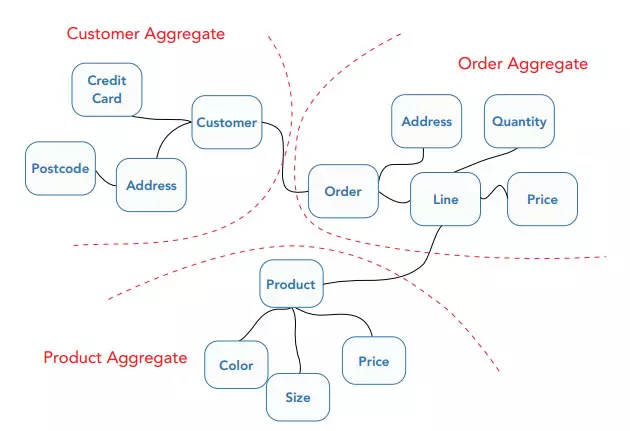
\includegraphics[width = 1\textwidth]{aggregate}
	\caption{Khuôn mẫu Aggregates}
\end{figure}

\subsubsection{Service}

Service là một lớp bổ sung cũng chứa logic nghiệp vụ. Nó là một phần của domain model, giống như các entity và value object. Đồng thời, dịch vụ ứng dụng là một lớp khác không chứa logic nghiệp vụ. Tuy nhiên, nó ở đây để điều phối hoạt động của ứng dụng, được đặt phía trên domain model.

Khi phân tích domain để xác định những đối tượng chính có trong mô hình, có thể bắt gặp những thành phần không dễ để có thể gán chúng cho một đối tượng nhất định nào đó. Tuy nhiên có một số hành vi trong domain lại không thuộc về một đối tượng nhất định nào cả. Chúng thể hiện cho những hành vi quan trọng trong domain nên không thể bỏ qua chúng hoặc gắn vào các Entity hay Value Object. Việc thêm hành vi này vào một đối tượng sẽ làm mất ý nghĩa của đối tượng đó, gán cho chúng những chức năng vốn không thuộc về chúng.

Đối với những hành vi như vậy trong domain, đó chính là một Service. Một Service không có trạng thái nội tại và nhiệm vụ của nó đơn giản là cung cấp các chức năng cho domain. Service có thể đóng một vai trò quan trọng trong domain, chúng có thể bao gồm các chức năng liên quan đến nhau để hỗ trợ cho các Entity và Value Object. Việc khai báo một Service một cách tường minh giúp phân biệt rõ các chức năng trong domain đó, giúp tách biệt rạch ròi khái niệm.

Một Service không nên bao gồm các thao tác vốn thuộc về các đối tượng của domain. Sẽ là không nên cứ có bất kỳ thao tác nào chúng ta cũng tạo một Service cho chúng. Chỉ khi một thao tác đóng một vai trò quan trọng trong domain ta mới cần tạo một Service để thực hiện.

\begin{figure}[H]
	\centering
	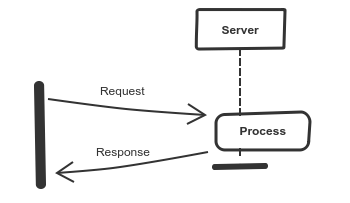
\includegraphics[width = 1\textwidth]{repository}
	\caption{Khuôn mẫu Service}
\end{figure}

\subsubsection{Repository}

Repository là một tập hợp các thực thể nghiệp vụ giúp đơn giản hóa cơ sở hạ tầng dữ liệu. Nó giải phóng domail model khỏi những lo ngại về cơ sở hạ tầng.

Mục đích của repository là để đóng gói tất cả các logic cần thiết để thu được các tham chiếu đối tượng. Các đối tượng domain sẽ không cần phải xử lý với cơ sở dữ liệu để lấy những tham chiếu cần thiết tới các đối tượng khác của domain. Chúng sẽ chỉ lấy nó từ Repository và model lấy lại được sự rõ ràng và tập trung.

Repository có thể lưu trữ các tham chiếu tới một vài đối tượng. Khi một đối tượng được khởi tạo, nó có thể được lưu lại trong Repository, và được lấy ra từ đây để có thể sử dụng sau này. Nếu phía client yêu cầu đối tượng từ Repository, và Repository không chứa chúng, nó có thể sẽ được lấy từ bộ nhớ. Dù bằng cách nào, các Repository hoạt động như một nơi lưu trữ các đối tượng cho việc truy xuất đối tượng toàn cục.

\begin{figure}[H]
	\centering
	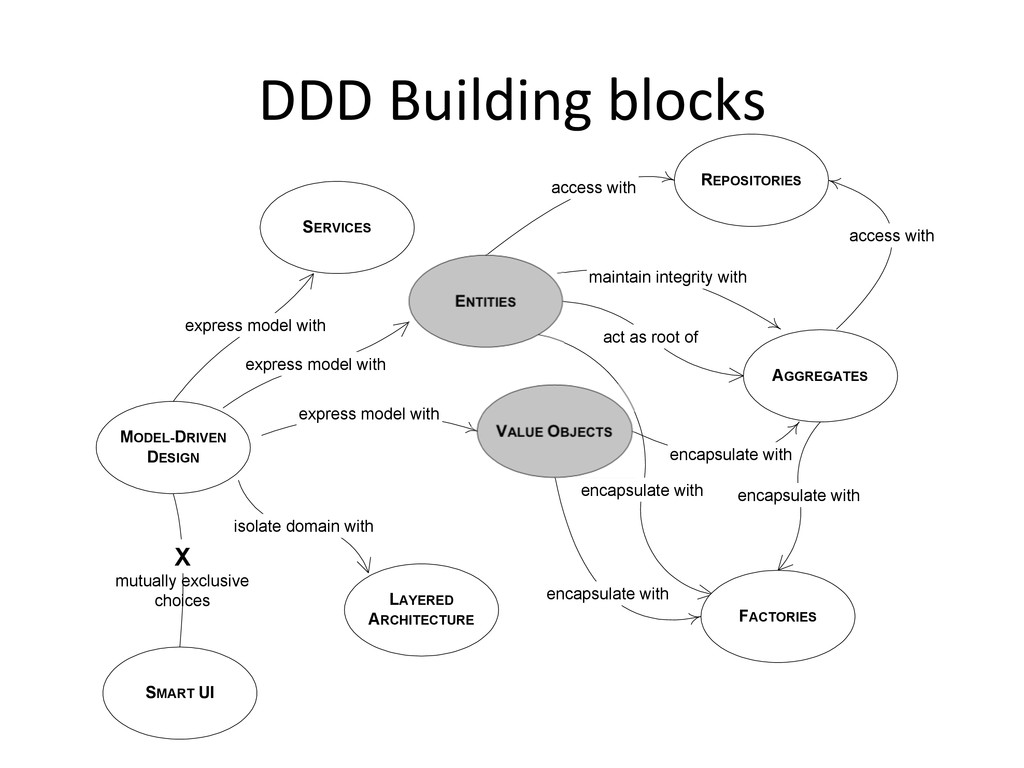
\includegraphics[width = 1\textwidth]{building-blocks}
	\caption{Các khuôn mẫu trong DDD}
\end{figure}

\subsection{Kiến trúc Onion}

Domain-driven design (DDD) là một cách tiếp cận để phát triển phần mềm cho các nhu cầu phức tạp bằng cách kết nối việc triển khai với một mô hình kinh doanh cốt lõi. DDD tập trung vào mô hình nghiệp vụ có hiểu biết phong phú về các quy trình và quy tắc của nghiệp vụ. Kiến trúc Onion thực hiện khái niệm này và tăng đáng kể chất lượng mã code, giảm độ phức tạp và cho phép các hệ thống doanh nghiệp phát triển.

Kiến trúc Onion được xây dựng trên mô hình nghiệp vụ trong đó các lớp được kết nối thông qua các interface. Ý tưởng là giữ các phụ thuộc bên ngoài càng xa càng tốt, nơi các thực thể nghiệp vụ và các quy tắc nghiệp vụ tạo thành phần cốt lõi của kiến trúc.

\begin{itemize}
	\item Nó cung cấp kiến trúc linh hoạt, bền vững và dễ mở rộng
	\item Các lớp được liên kết chặt chẽ và có sự phân tách rõ ràng
	\item Nó cung cấp khả năng bảo trì tốt hơn vì tất cả mã code phụ thuộc vào các lớp sâu hơn hoặc lớp trung tâm
	\item Cải thiện khả năng kiểm tra vì các kiểm tra có thể được tạo cho các lớp riêng biệt mà không ảnh hưởng đến các lớp khác
	\item Các công nghệ có thể dễ dàng thay đổi mà không ảnh hưởng đến nghiệp vụ lõi
\end{itemize}

Các tầng được biểu diễn thành dạng các vòng tròn đồng tâm. Đặc trưng của kiến trúc củ hành đó là một luật về sự ràng buộc giữa các tầng. Tầng bên ngoài chỉ phụ thuộc và gọi trực tiếp tầng bên trong. Các tầng thấp hơn không thể phụ thuộc vào các tầng bên ngoài.

\subsubsection{Nguyên lý}

Kiến trúc Onion bao gồm nhiều lớp đồng tâm giao thoa với nhau về phía lõi đại diện cho nghiệp vụ. Nó dựa trên sự đảo ngược của nguyên tắc điều khiển. Kiến trúc không tập trung vào công nghệ hay khuôn khổ mà là các mô hình nghiệp vụ thực tế. Nó dựa trên các nguyên tắc sau:

\begin{itemize}
	\bfitem{Sự phụ thuộc}{Các vòng tròn đại diện cho các lớp trách nhiệm khác nhau. Nói chung, càng đi sâu, các lớp càng tiến gần đến nghiệp vụ và các quy tắc kinh doanh. Các lớp bên ngoài đại diện cho các cơ chế và các lớp bên trong đại diện cho logic nghiệp vụ. Các lớp bên ngoài phụ thuộc vào các lớp bên trong và các lớp bên trong hoàn toàn không nhận biết được các lớp bên ngoài. Định dạng / cấu trúc dữ liệu có thể khác nhau giữa các lớp. Các định dạng dữ liệu lớp bên ngoài không được sử dụng bởi các lớp bên trong}
	\bfitem{Bao bọc dữ liệu}{Mỗi lớp bao bọc hoặc ẩn các chi tiết triển khai bên trong và cung cấp API cho lớp bên ngoài. Tất cả các lớp cũng cần cung cấp thông tin để cho các lớp bên trong sử dụng một cách thuận tiện. Mục đích là giảm thiểu sự kết hợp giữa các lớp và tối đa hóa sự kết hợp trong một lát dọc giữa các lớp. Điều này đảm bảo sự tập trung vào mô hình nghiệp vụ mà không cần lo lắng quá nhiều về chi tiết triển khai}
	\bfitem{Tách mối quan tâm}{Ứng dụng được chia thành các lớp trong đó mỗi lớp có một tập hợp các trách nhiệm và giải quyết các mối quan tâm riêng biệt. Mỗi lớp hoạt động như các modules/package/namespace tên trong ứng dụng}
	\bfitem{Rằng buộc}{Rằng buộc thấp trong đó một module tương tác với một module khác và không cần quan tâm đến các phần bên trong của module đó. Tất cả các lớp bên trong không cần quan tâm đến việc triển khai của các lớp bên ngoài}
\end{itemize}

\subsubsection{Các lớp của Kiến trúc Onion}

\begin{itemize}
	\bfitem{Lớp nghiệp vụ}{Ở phần trung tâm của Kiến trúc Onion, lớp miền tồn tại; lớp này đại diện cho các đối tượng nghiệp vụ và hành vi. Ý tưởng là có tất cả các đối tượng miền của bạn ở cốt lõi này. Nó chứa tất cả các đối tượng miền ứng dụng. Bên cạnh các đối tượng miền, bạn cũng có thể có các giao diện miền. Các thực thể miền này không có bất kỳ phụ thuộc nào}
	\bfitem{Lớp kho lưu trữ}{Lớp này tạo ra một sự trừu tượng giữa các thực thể miền và logic nghiệp vụ của một ứng dụng. Trong lớp này, thường thêm các giao diện cung cấp hành vi lưu và truy xuất đối tượng thường bằng cách liên quan đến cơ sở dữ liệu. Lớp này bao gồm mẫu truy cập dữ liệu, là một cách tiếp cận kết hợp lỏng hơn để truy cập dữ liệu. Chúng tôi cũng tạo một kho lưu trữ chung và thêm các truy vấn để truy xuất dữ liệu từ nguồn, ánh xạ dữ liệu từ nguồn dữ liệu sang một thực thể kinh doanh và duy trì những thay đổi trong thực thể kinh doanh đối với nguồn dữ liệu}
	\bfitem{Lớp dịch vụ}{Lớp Dịch vụ giữ các giao diện với các hoạt động phổ biến, chẳng hạn như Thêm, Lưu, Chỉnh sửa và Xóa. Ngoài ra, lớp này được sử dụng để giao tiếp giữa lớp UI và lớp kho lưu trữ. Lớp Dịch vụ cũng có thể giữ logic nghiệp vụ cho một thực thể. Trong lớp này, các giao diện dịch vụ được giữ với quá trình triển khai của nó, giữ cho sự liên kết lỏng và tách biệt các mối quan tâm trong tâm trí}
	\bfitem{Lớp giao diện người dùng}{Đây là lớp ngoài cùng và giữ các mối quan tâm ngoại vi như giao diện người dùng và các thử nghiệm. Đối với một ứng dụng Web, nó đại diện cho dự án Web API hoặc Unit Test. Lớp này có sự triển khai của nguyên tắc tiêm phụ thuộc để ứng dụng xây dựng một cấu trúc liên kết lỏng và có thể giao tiếp với lớp bên trong thông qua các giao diện}
\end{itemize}

\begin{figure}[H]
	\centering
	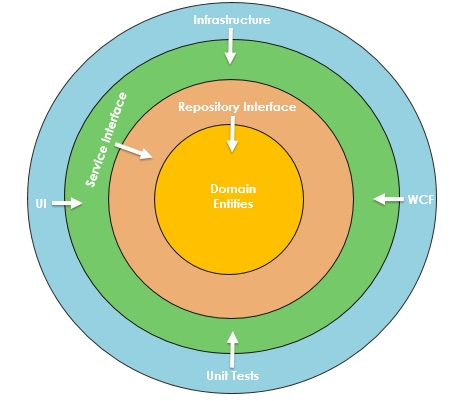
\includegraphics[width = 0.7\textwidth]{onion_architecture}
	\caption{Các lớp của Kiến trúc Onion}
\end{figure}

\section{Kiến trúc tổng quan hệ thống}

\subsection{Hệ thống frontend}

\subsubsection{Hệ thống Trang}

Hệ thống frontend có các hệ thống Trang sau đây: Product, Layer, Experiment và Test Group. Mỗi hệ thống Trang bao gồm có hệ thống Đường dẫn, mỗi Đường dẫn có một nhiệm vụ cụ thể được ghi chú trong Chú thích.

Mỗi thực thể đều có một hệ thống Trang nhằm mục đích cho người dùng có thể khởi tạo, cập nhập và thay đổi theo ý muốn. Ngoài ra người dùng có thể có cái nhìn toàn cảnh với mỗi thực thể.

\begin{table}[H]
	\centering
	\begin{tabular}{|c|l|p{5cm}|}
		\hline
		Trang                    & Đường dẫn                                       & Chú thích                \\ \hline
		\multirow{4}{*}{Product} & /product                                        & Hiển thị toàn bộ Product \\ \cline{2-3}
		                         & /product/new                                    & Khởi tạo Product         \\ \cline{2-3}
		                         & /product/:id                                    & Hiển thị Product         \\ \cline{2-3}
		                         & /product/:id/update                             & Cập nhật Product         \\ \hline
		\multirow{4}{*}{Layer}
		                         & /product/:id/layer/new                          & Khởi tạo Layer           \\ \cline{2-3}
		                         & /product/:id/layer/:id                          & Hiển thị Layer           \\ \cline{2-3}
		                         & /product/:id/layer/:id/update                   & Cập nhật Layer           \\ \hline
		\multirow{4}{*}{Experiment}
		                         & /product/:id/layer/:id/exp/new                  & Khởi tạo Experiment      \\ \cline{2-3}
		                         & /product/:id/layer/:id/exp/:id                  & Hiển thị Layer           \\ \cline{2-3}
		                         & /product/:id/layer/:id/exp/:id/update           & Cập nhật Layer           \\ \hline
		\multirow{4}{*}{Group}
		                         & /product/:id/layer/:id/exp/:id/group/new        & Khởi tạo Test Group      \\ \cline{2-3}
		                         & /product/:id/layer/:id/exp/:id/group/:id        & Hiển thị Test Group      \\ \cline{2-3}
		                         & /product/:id/layer/:id/exp/:id/group/:id/update & Cập nhật Test Group      \\ \hline
	\end{tabular}
	\caption{Hệ thống Trang}
\end{table}

Với mỗi Trang, các thông tin sẽ được hiển thị như sau:

\begin{itemize}
	\bfitem{/product}{}
	\begin{itemize}
		\item Toàn bộ Product
		\item Id của mỗi Product
		\item Tên của mỗi Product
		\item Số lượng Layer trong mỗi Product
	\end{itemize}
	\bfitem{/product/:id}{}
	\begin{itemize}
		\item Tên của Product
		\item Số lượng Layer của Product
		\item Số lượng Experiment của Product
		\item Toàn bộ Layer của Product
		      \begin{itemize}
			      \item Id của mỗi Layer
			      \item Tên của mỗi Layer
			      \item Hash stragety của mỗi Layer
			      \item Số lượng Experiment của mỗi Layer
		      \end{itemize}
	\end{itemize}
	\bfitem{/product/:id/layer/:id}{}
	\begin{itemize}
		\item Tên của Layer
		\item Hash stragety của Layer
		\item Traffic còn lại của Layer
		\item Số lượng Experiment của Layer
		\item Toàn bộ Experiment của Layer
		      \begin{itemize}
			      \item Id của mỗi Experiment
			      \item Tên của mỗi Experiment
			      \item Traffic của mỗi Experiment
			      \item Trạng thái của mỗi Experiment
			      \item Thời điểm bắt đầu của mỗi Experiment
			      \item Thời điểm kết thúc của mỗi Experiment
			      \item Số lượng Test Group của mỗi Experiment
		      \end{itemize}
	\end{itemize}
	\bfitem{/product/:id/layer/:id/exp/:id}{}
	\begin{itemize}
		\item Tên của Experiment
		\item Traffic của Experiment
		\item Trạng thái của Experiment
		\item Thời điểm bắt đầu của Experiment
		\item Thời điểm kết thúc của Experiment
		\item Số lượng Test Group của Experiment
		\item Toàn bộ Test Group của Experiment
		      \begin{itemize}
			      \item Id của mỗi Test Group
			      \item Tên của mỗi Test Group
			      \item Toàn bộ Parameter của Test Group
			            \begin{itemize}
				            \item Tên của mỗi Parameter
				            \item Giá trị của mỗi Parameter
			            \end{itemize}
		      \end{itemize}
	\end{itemize}
\end{itemize}

\subsubsection{Các thành phần}

Hệ thống frontend gồm các thành phần sau: Types, Pages, Services và Components

\begin{itemize}
	\bfitem{Types}{Mục đích là tổng hợp các thực thể ở tầng Frontend, bao gồm hai loại là Thực thể gốc và nội dung khi nhận/gửi API}
	\bfitem{Pages}{Là thành phần xử lý hệ thống Trang, mỗi file sẽ là một hệ thống Trang khác nhau}
	\bfitem{Services}{Là thành phần xử lý hệ thống thông tin cho toàn bộ hệ thống Frontend, bao gồm cả việc nhận, gửi dữ liệu từ Server}
	\bfitem{Components}{Chứa các thành phần chung giữa các trang}
\end{itemize}

% \begin{figure}[H]
% 	\centering
% 	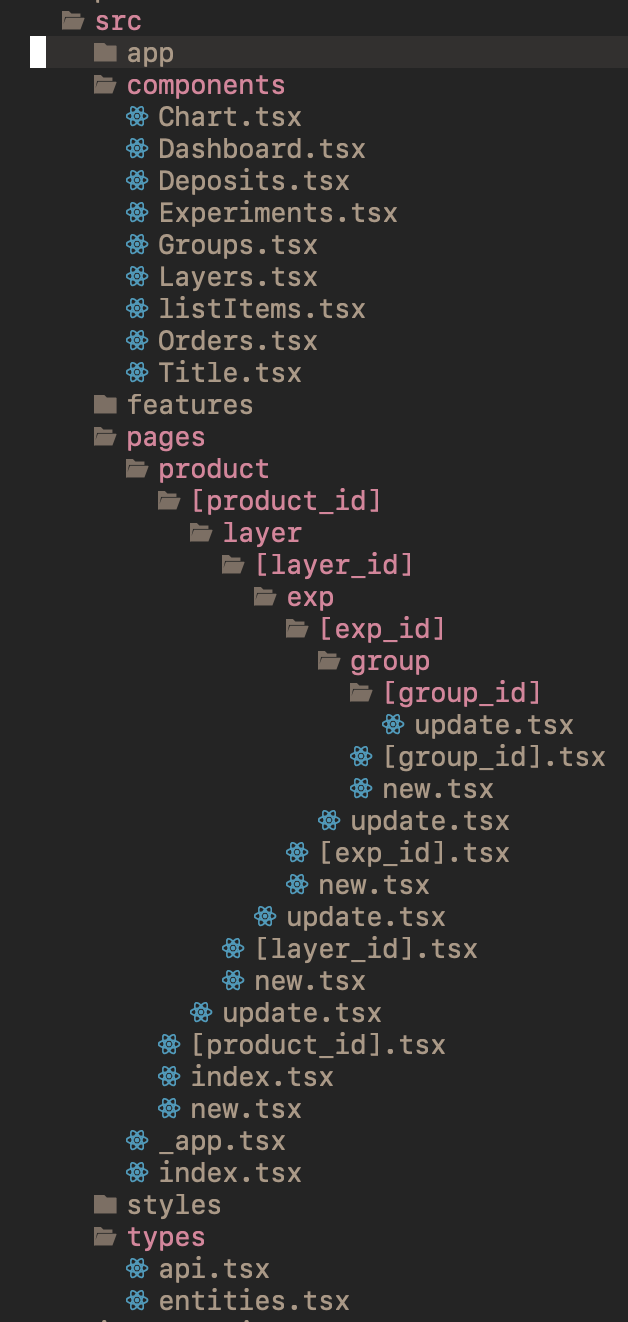
\includegraphics[width = 0.7\textwidth]{frontend-structure}
% 	\caption{Hệ thống Frontend}
% \end{figure}

\subsection{Hệ thống backend}

\subsubsection{Các thành phần}

Các thành phần trong hệ thống backend đảm nhiệm một nhiệm vụ riêng biệt gồm các thành phần sau:

\begin{itemize}
	\bfitem{Service}{Là thành phần xử lý hệ thống HTTP, chuyên nhận và phản hồi các truy cập từ hệ thống Frontend}
	\begin{itemize}
		\bfitem{Summary}{Gửi trả toàn bộ dữ liệu của các A/B Test}
		\bfitem{Abtest}{Thực hiện và gửi trả A/B Test}
		\bfitem{Entity}{Thực hiện khởi tạo hoặc cập nhật các thực thể, gửi trả kết quả}
	\end{itemize}
	\bfitem{Storage}{Là thành phần tổng hợp thông tin cho tầng Service}
	\begin{itemize}
		\bfitem{Summary}{Tổng hợp toàn bộ dữ liệu của các A/B Test}
		\bfitem{Entity}{Khởi tạo hoặc cập nhật các thực thể}
	\end{itemize}
	\bfitem{Database}{Là thành phần quản lý dữ liệu cho tầng Storage}
	\begin{itemize}
		\bfitem{Entity}{Khởi tạo hoặc cập nhật các thực thể}
	\end{itemize}
	\bfitem{Types}{Tổng hợp các thực thể ở tầng Backend, bao gồm 2 loại là: thực thể gốc và nội dung khi nhận/gửi API}
	\begin{itemize}
		\bfitem{Entity}{Dữ liệu của các thực thể}
		\bfitem{API}{Dữ liệu nội dung cho các yêu cầu/kết quả khi truy cập}
	\end{itemize}
	\bfitem{Abtest}{Thực hiện A/B Test}
\end{itemize}

\begin{figure}[H]
	\centering
	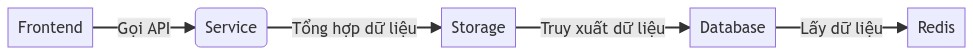
\includegraphics[width = 1\textwidth]{backend}
	\caption{Hệ thống Backend}
\end{figure}

\subsubsection{Hệ thống API}

Mỗi thực thể có chức năng riêng biệt nhau. Hệ thống đường dẫn bao gồm các thực thể sau:

\begin{table}[H]
	\centering
	\begin{tabular}{|l|l|l|}
		\hline
		\textbf{Thực thể}           & \textbf{Đường dẫn} & \textbf{Chú thích}                          \\ \hline
		Summary                     & /summary           & Gọi toàn bộ thông tin của hệ thống A/B Test \\ \hline
		AbTest                      & /abtest            & Thực hiện A/B Test                          \\ \hline
		\multirow{2}{*}{Product}    & /product/create    & Khởi tạo Product mới                        \\ \cline{2-3}
		                            & /product/update    & Cập nhật Product                            \\ \hline
		\multirow{2}{*}{Layer}      & /layer/create      & Khởi tạo Layer mới                          \\ \cline{2-3}
		                            & /layer/update      & Cập nhật Layer                              \\ \hline
		\multirow{2}{*}{Experiment} & /exp/create        & Khởi tạo Experiment mới                     \\ \cline{2-3}
		                            & /exp/update        & Cập nhật Experiment                         \\ \hline
		\multirow{2}{*}{Test Group} & /group/create      & Khởi tạo Test Group mới                     \\ \cline{2-3}
		                            & /group/update      & Cập nhật Test Group mới                     \\ \hline
	\end{tabular}
	\caption{Hệ thống đường dẫn}
\end{table}

Với mỗi API, sẽ có cấu trúc về yêu cầu và kết quả như sau:

\begin{itemize}
	\bfitem{Summary}{}
	\begin{itemize}
		\bfitem{Kết quả}{Toàn bộ Product, trong Product có toàn bộ Layer của Product đó, v.v}
	\end{itemize}
	\bfitem{AbTest}{}
	\begin{itemize}
		\bfitem{Yêu cầu}{Thông tin của user và product nào cần thực hiện A/B Test}
		\begin{itemize}
			\bfitem{product id}{Id của Product cần thực hiện A/B Test}
			\bfitem{user id}{Id của người dùng}
			\bfitem{session id}{Id của sesion mà người dùng đang sử dụng}
		\end{itemize}
		\bfitem{Kết quả}{Thông tin của các A/B Test thử nghiệm với user}
		\begin{itemize}
			\bfitem{product id}{Id của Product đang thực hiện A/B Test}
			\bfitem{layer id}{Id của Layer sẽ thực hiện A/B Test này}
			\bfitem{experiment id}{Id của Experiment sẽ thực hiện A/B Test này}
			\bfitem{test group id}{Id của Test Group sẽ thực hiện A/B Test này}
			\bfitem{parameters}{Tên và giá trị của các Parameter}
		\end{itemize}
	\end{itemize}
	\bfitem{Product}{}
	\begin{itemize}
		\bfitem{Create}{Khởi tạo một Product}
		\begin{itemize}
			\bfitem{Yêu cầu}{Nội dung của Product đó}
			\bfitem{Kết quả}{Nội dung của Product đó cộng thêm mã id định danh}
		\end{itemize}
		\bfitem{Update}{Cập nhật một Product}
		\begin{itemize}
			\bfitem{Yêu cầu}{Nội dung của Product đó}
			\bfitem{Kết quả}{Nội dung của Product đó}
		\end{itemize}
	\end{itemize}
	\bfitem{Layer}{}
	\begin{itemize}
		\bfitem{Create}{Khởi tạo một Layer}
		\begin{itemize}
			\bfitem{Yêu cầu}{Nội dung của Layer đó}
			\bfitem{Kết quả}{Nội dung của Layer đó cộng thêm mã id định danh}
		\end{itemize}
		\bfitem{Update}{Cập nhật một Layer}
		\begin{itemize}
			\bfitem{Yêu cầu}{Nội dung của Layer đó}
			\bfitem{Kết quả}{Nội dung của Layer đó}
		\end{itemize}
	\end{itemize}
	\bfitem{Experiment}{}
	\begin{itemize}
		\bfitem{Create}{Khởi tạo một Experiment}
		\begin{itemize}
			\bfitem{Yêu cầu}{Nội dung của Experiment đó}
			\bfitem{Kết quả}{Nội dung của Experiment đó cộng thêm mã id định danh}
		\end{itemize}
		\bfitem{Update}{Cập nhật một Experiment}
		\begin{itemize}
			\bfitem{Yêu cầu}{Nội dung của Experiment đó}
			\bfitem{Kết quả}{Nội dung của Experiment đó}
		\end{itemize}
	\end{itemize}
	\bfitem{Test Group}{}
	\begin{itemize}
		\bfitem{Create}{Khởi tạo một Test Group}
		\begin{itemize}
			\bfitem{Yêu cầu}{Nội dung của Test Group đó}
			\bfitem{Kết quả}{Nội dung của Test Group đó cộng thêm mã id định danh}
		\end{itemize}
		\bfitem{Update}{Cập nhật một Test Group}
		\begin{itemize}
			\bfitem{Yêu cầu}{Nội dung của Test Group đó}
			\bfitem{Kết quả}{Nội dung của Test Group đó}
		\end{itemize}
	\end{itemize}
\end{itemize}

\subsection{Biểu đồ tuần tự}

\subsubsection{Biểu đồ tuần tự chung}

Biểu đồ tuần tự chung biểu thị việc khởi tạo và sử dụng A/B Test.

\begin{figure}[H]
	\centering
	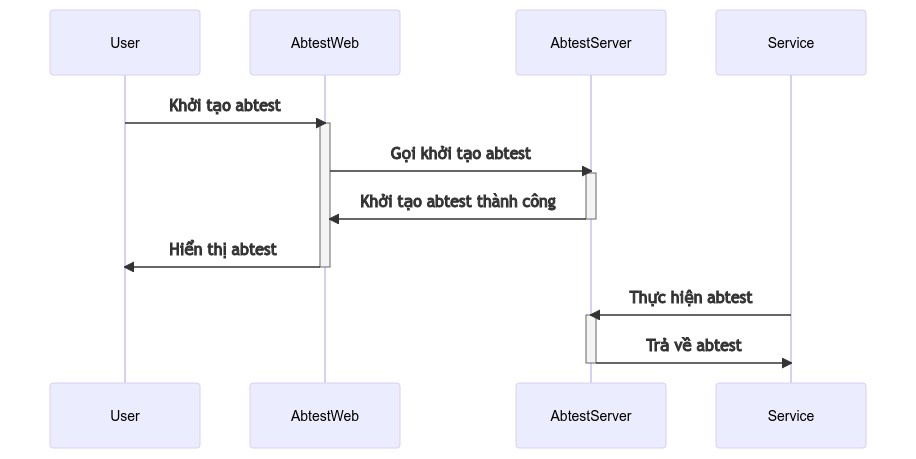
\includegraphics[width = 1\textwidth]{overview-sequence}
	\caption{Biểu đồ tuần tự chung}
\end{figure}

\subsubsection{Biểu đồ tuần tự khởi tạo A/B Test}

Biểu đồ tuần tự khởi tạo A/B Test

\begin{figure}[H]
	\centering
	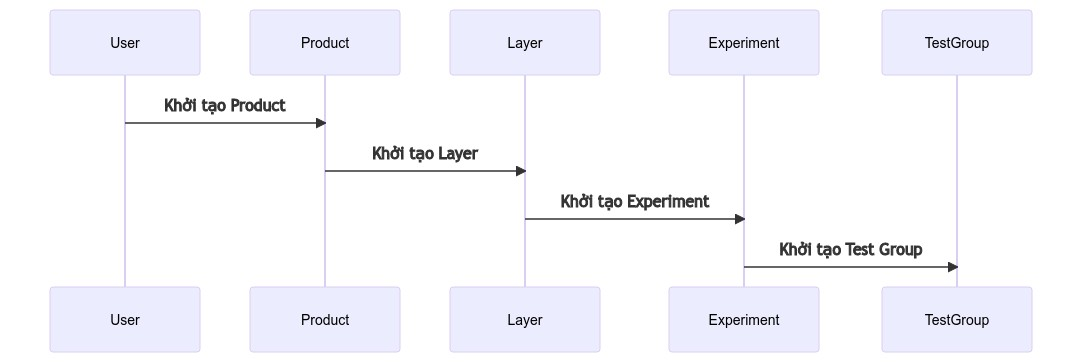
\includegraphics[width = 1\textwidth]{abtest-sequence}
	\caption{Biểu đồ tuần tự khởi tạo A/B Test}
\end{figure}

\section{Mô hình cơ sở dữ liệu}

Mô hình cơ sở dữ liệu của hệ thống mô tả cụ thể các đặc tính của mỗi thực thể, ngoài ra mô tả
cách lưu trữ các thực thể và các mối quan hệ tương quan trong cơ sở dữ liệu.

\subsection{Các thực thể}

Các thực thể bao gồm: Product, Layer, Experiment và Test Group.

\subsubsection{Product}

Product là thực thể lớn nhất, chỉ có chức năng phân tách theo nhu cầu sử dụng nên chỉ có 2 trường như sau:
\begin{table}[H]
	\centering
	\begin{tabular}{|l|l|l|}
		\hline
		Trường & Loại   & Chú thích       \\ \hline
		id     & int    & Mã id định danh \\ \hline
		name   & string & Tên của Product \\ \hline
	\end{tabular}
	\caption{Thuộc tính của Product}
\end{table}

Cấu hình khi được lưu xuống cơ sở dữ liệu:

\begin{itemize}
	\bfitem{Key}{product::[id]}
	\bfitem{Value}{binary (nén bởi JSON)}
	\bfitem{Command}{SET, GET}
\end{itemize}

\subsubsection{Layer}

\begin{table}[H]
	\centering
	\begin{tabular}{|l|l|l|}
		\hline
		Trường & Loại   & Chú thích       \\ \hline
		id     & int    & Mã id định danh \\ \hline
		name   & string & Tên của Layer   \\ \hline
		type   & int    & Loại của Layer  \\ \hline
	\end{tabular}
	\caption{Thuộc tính của Layer}
\end{table}

Cấu hình khi được lưu xuống cơ sở dữ liệu:

\begin{itemize}
	\bfitem{Key}{layer::[id]}
	\bfitem{Value}{binary (nén bởi JSON)}
	\bfitem{Command}{SET, GET}
\end{itemize}

\subsubsection{Experiment}

\begin{table}[H]
	\centering
	\begin{tabular}{|l|l|l|}
		\hline
		Trường      & Loại   & Chú thích          \\ \hline
		id          & int    & Mã id định danh    \\ \hline
		name        & string & Tên của Experiment \\ \hline
		traffic     & int    & Số lượng traffic   \\ \hline
		start\_time & int    & Thời điểm bắt đầu  \\ \hline
		end\_time   & int    & Thời điểm kết thúc \\ \hline
		status      & int    & Trạng thái         \\ \hline
	\end{tabular}
	\caption{Thuộc tính của Experiment}
\end{table}

Cấu hình khi được lưu xuống cơ sở dữ liệu:

\begin{itemize}
	\bfitem{Key}{exp::[id]}
	\bfitem{Value}{binary (nén bởi JSON)}
	\bfitem{Command}{SET, GET}
\end{itemize}

\subsubsection{Test Group}

\begin{table}[H]
	\centering
	\begin{tabular}{|l|l|l|}
		\hline
		Trường    & Loại   & Chú thích                \\ \hline
		id        & int    & Mã id định danh          \\ \hline
		parameter & string & Parameter của Test Group \\ \hline
		value     & string & Value của Parameter      \\ \hline
	\end{tabular}
	\caption{Thuộc tính của Test Group}
\end{table}

Cấu hình khi được lưu xuống cơ sở dữ liệu:

\begin{itemize}
	\bfitem{Key}{group::[id]}
	\bfitem{Value}{binary (nén bởi JSON)}
	\bfitem{Command}{SET, GET}
\end{itemize}

\subsection{Mối quan hệ giữa các thực thể}

Giữa các thực thể có các mối quan hệ lẫn nhau, vì vậy ngoài việc lưu trữ các thực thể dưới
cơ sở dữ liệu, cũng cần lưu trữ mối quan hệ giữa chúng.

\subsubsection{Tổng hợp các Product}

Khi cần query tất cả các Product hiện có, chỉ cần lưu các id của product vào một chỗ.

Cấu hình khi được lưu xuống cơ sở dữ liệu:

\begin{itemize}
	\bfitem{Key}{product::ids}
	\bfitem{Value}{các id của product}
	\bfitem{Command}{SADD, SMEMBERS}
\end{itemize}

\subsubsection{Giữa Product và Layer}

Mỗi Product có nhiều Layer, khi cần query tất cả các Layer dưới một Product, chỉ cần lưu
các id của layer vào một chỗ.

Cấu hình khi được lưu xuống cơ sở dữ liệu:

\begin{itemize}
	\bfitem{Key}{product::[id]::layers}
	\bfitem{Value}{các id của Layer}
	\bfitem{Command}{SADD, SMEMBERS}
\end{itemize}

\subsubsection{Giữa Layer và Experiment}

Mỗi Layer có nhiều Experiment, khi cần query tất cả các Experiment dưới một Layer, chỉ cần lưu
các id của Experiment vào một chỗ.

Cấu hình khi được lưu xuống cơ sở dữ liệu:

\begin{itemize}
	\bfitem{Key}{layer::[id]::exps}
	\bfitem{Value}{các id của Experiment}
	\bfitem{Command}{SADD, SMEMBERS}
\end{itemize}

\subsubsection{Giữa Experiment và Test Group}

Mỗi Experiment có nhiều Test Group, khi cần query tất cả các Test Group dưới một Experiment, chỉ cần lưu
các id của Test Group vào một chỗ.

Cấu hình khi được lưu xuống cơ sở dữ liệu:

\begin{itemize}
	\bfitem{Key}{exp::[id]::groups}
	\bfitem{Value}{các id của Test Group}
	\bfitem{Command}{SADD, SMEMBERS}
\end{itemize}

\subsection{Id Generator}

Mỗi thực thể đều yêu cầu một mã ID định danh, do đó cơ sở dữ liệu cũng cần được sử dụng để mỗi
khi tạo một thực thể mới có thể có một mã ID định danh mới.

Cấu hình khi được lưu xuống cơ sở dữ liệu:

\begin{itemize}
	\bfitem{Key}{product::id, layer::id, exp::id, group::id}
	\bfitem{Value}{Mã ID đang sử dụng hiện tại}
	\bfitem{Command}{INCR}
\end{itemize}
